%% Cahpter_Zusammenfassung.tex
%%

%% ===========================
\chapter{Fazit und Ausblick}
\label{ch:Ergebnis}
%% ===========================

In diesem abschließenden Kapitel werden die Ergebnisse der Arbeit in ihren wichtigsten Punkten zusammengefasst und anhand der Anforderungen aus Kapitel \ref{ch:Systemanalyse:sec:Anforderungsanalyse} bewertet. Anschließend wird ein Ausblick auf weiterführende Möglichkeiten, sowie zukünftige Verbesserungsmöglichkeiten gegeben. 

%% ===========================
\section{Zusammenfassung}
\label{ch:Ergebnis:sec:zusammenfassung}
%% ===========================

Aus der Motivation heraus wurde in der vorliegenden Arbeit ein System, basierend auf den Daten von CAS genesisWorld entwickelt. Hierzu wurden zuerst alle relevanten Komponenten von CAS genesisWorld untersucht. Dabei wurden Tabellen und Spalten identifiziert, die zur Realisierung der Lösung notwendig sind. Anschließend wurden die Anforderungen an das neue System erhoben. Mit dem Wissen über die zu übernehmenden Daten und den Anforderungen wurde eine passende Datenbank ausgewählt. Diese sollte den zuvor erhobenen Anforderungen gerecht werden. Dabei wurden NoSQL-Datenbanken hinsichtlich ihrer Eignung untersucht. Sie konnten in diesem Fall allerdings nicht überzeugen, somit entschied man sich für die H2-Datenbank. Die Entscheidung zugunsten der H2-Datenbank ist auf die im Hauptspeicher gehaltenen Tabellen zurückzuführen.   

Aufbauend auf der zuvor ausgewählten Datenbank wurden Konzepte zur Umsetzung des Systems entwickelt. Bei der Konzeption wurde deduktiv vorgegangen. Zuerst wurde die Architektur definiert und anschließend die einzelnen Komponenten detailliert geplant. Bei der Planung wurde nicht versucht ein universell einsetzbares System zu entwickeln, sondern vielmehr eine domänenspezifische Lösung für das Szenario auszuarbeiten. Nachdem alle Technologien, sowie Vorgehensweisen festgelegt wurden, ging man auf die Umsetzungen ein. Indessen eine Beschreibung der Funktionsweise einzelner Komponenten durchgeführt wurde. Neben der Funktionsweise wurde die Interaktion unter den Komponenten dargelegt. Schlussendlich wurde die fertige Oberfläche und die getroffenen Designentscheidungen dargelegt.
 
%% ===========================
\section{Bewertung der Ergebnisse}
\label{ch:Ergebnis:sec:bewertung}
%% ===========================

Die funktionalen Anforderungen konnten alle umgesetzt werden und wurden bereits im vorherigen Kapitel anhand der Oberfläche erläutert. Im Folgenden wird somit auf die Erfüllung der nicht funktionalen Anforderungen eingegangen. Dies erfolgt anhand der Gegenüberstellung von Anforderungen und den Charakteristika des Systems.

Die erste Anforderung konnte durch den Betrieb auf einem Server eingehalten werden. Weiterhin wurde eine lose Kopplung erreicht. Diese spiegeln sich in den REST-Schnittstellen der jeweiligen Komponenten wieder. Überdies gibt es keine Abhängigkeiten zwischen den Klassen der Darstellung und den Klassen der Geschäftslogik. Ein gewisses Maß an Portabilität wurde vorausgesetzt, damit ein verlagern des Systems auf andere Instanzen kein Problem darstellt. Dies wurde durch die Verwendung der Web-Archive-Dateien erreicht. Sie ermöglichen den Einsatz auf verschiedenen Tomcat Servern, was sie nicht nur portabel macht, sondern auch verschiedenen Servern einsetzbar macht. 

Einer der wichtigsten Anforderungen ist die geringe Abfragegeschwindigkeit. Tabelle \ref{tb:vergleichAbfragegeschwindigkeit} zeigt, dass dieser Forderung nachgekommen wird. Ebenfalls deutlich zu erkennen ist die Auswirkung des geänderten Schemas. Der Sprung von 98.000 ms auf 350 ms ist durch die Reduktion in der Abfragekomplexität zu erklären. Die Abfragen erfolgen über wesentlich weniger Tabellen und Spalten als zuvor. Außerdem wird im neuen Schema kein Verbund in der Datenbankabfrage mehr benötigt. Allerdings sind bei derartigen Maßnahmen, wie sie im Schemadesign ergriffen wurden, weitreichende Folgen zu beachten. Eine davon ist eine sehr schlechte Erweiterbarkeit des Schemas. Im momentanen Schema können lediglich Spalten hinzugezogen werden, dessen Inhalt in allen Verbindungsmerkmalen vorhanden ist. Außerdem würden für jede weitere Spalte, 18 Mio. zusätzliche Werte entstehen. Die Hinzunahme von merkmalspezifischen Attributen würde ebenfalls zu hohen Änderungsaufwänden führen. Als eine Konsequenzen müsste die \textit{data} Tabelle in mehrere Tabellen aufgeteilt werden. Dies würde eine stärke Normalisierung des Schemas bewirken und den Einsatz von Verbundoperatoren erfordern. Dadurch würde die Verarbeitungsgeschwindigkeit bei Lesezugriffen steigen. Allerdings wären dennoch wesentlich weniger Verbundoperatoren als im alten Schema nötig. Aufgrund dessen ist trotzdem mit einer deutlichen geringeren Abfragegeschwindigkeit als in CAS genesisWorld zu rechnen.  

\begin{table}[htbp]
\centering
\begin{tabular} {l | r}
Versuchskomponente & Zeit in ms  \\ \hline
MSSQL Datenbank \& Altes Schema & 98000 \\
MSSQL Datenbank \& Neues Schema & 350 \\
H2 Datenbank \& Neues Schema & 80 \\
\end{tabular}
\caption{Abfragegeschwindigkeit Vergleich}
\label{tb:vergleichAbfragegeschwindigkeit}
\end{table}

Nachdem Änderungen welche eine Steigerung der Komplexität bewirken betrachtet wurden, stellt sich folgende Frage: Ist die Datenbank nur aufgrund des geänderten Schemas deutlich schneller? Um dieser Frage nachzugehen wurden Tests durchgeführt. Abbildung \ref{ergebniss_vergleich} zeigt die Ergebnisse dieser Testreihen. Alle Testläufe wurden auf einem Client durchgeführt. Dieser simulierte mithilfe von Multithreading den Zugriff von 100 gleichzeitigen Benutzern. Die in den Diagrammen angegebene Zeit bezieht sich somit auf die Ausführung aller 100 Abfragen. Jeder simulierte Benutzer führt die auf der y Achse angegebene Anweisung aus. Beim obersten Balken in (a) sind es beispielsweise 15 Mio. SELECT-Anweisungen pro Benutzer. In (b) hingegen wird die Verarbeitungsgeschwindigkeit bei Updates verglichen. Der Vergleich anhand von Insert-Anweisungen wird in (c] gezeigt.    

\begin{figure}[htbp]
\centering
\subfigure[Vergleich anhand Select-Performance]{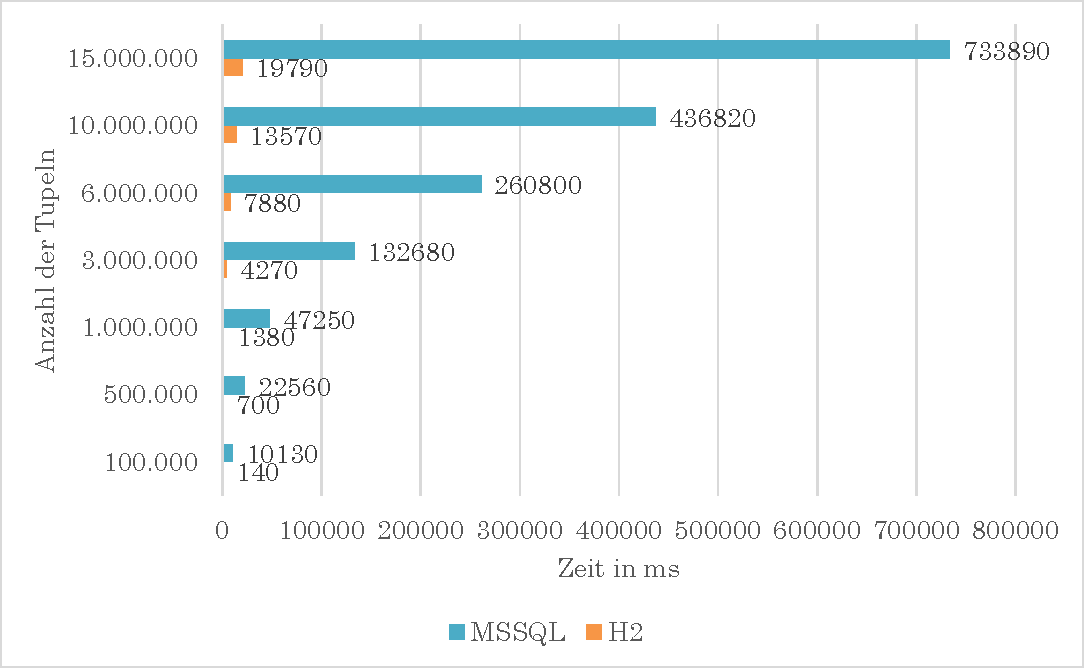
\includegraphics[width=0.49\textwidth]{charts/select.pdf}}\hfill
\subfigure[Vergleich anhand Update-Performance]{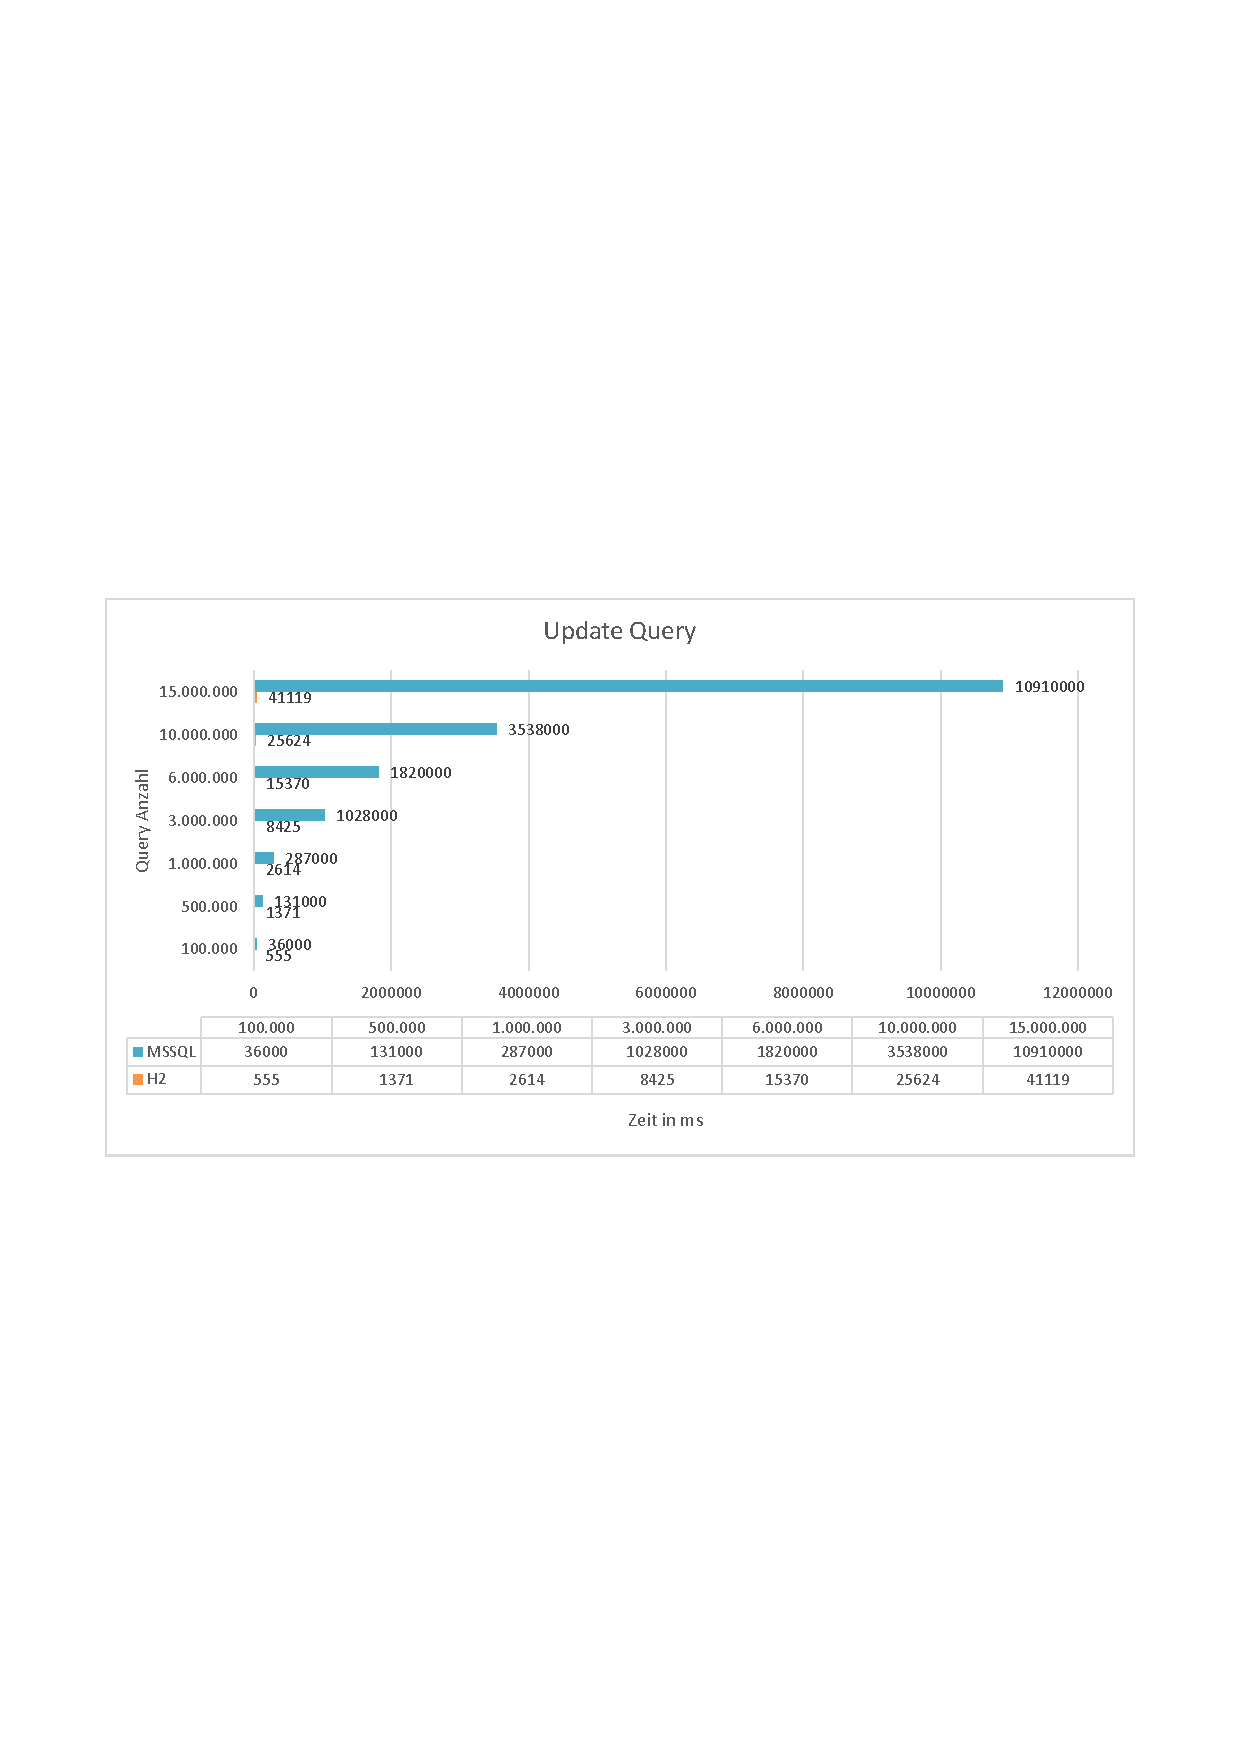
\includegraphics[width=0.49\textwidth]{charts/update.pdf}}\hfill
\subfigure[Vergleich anhand Insert-Performance]{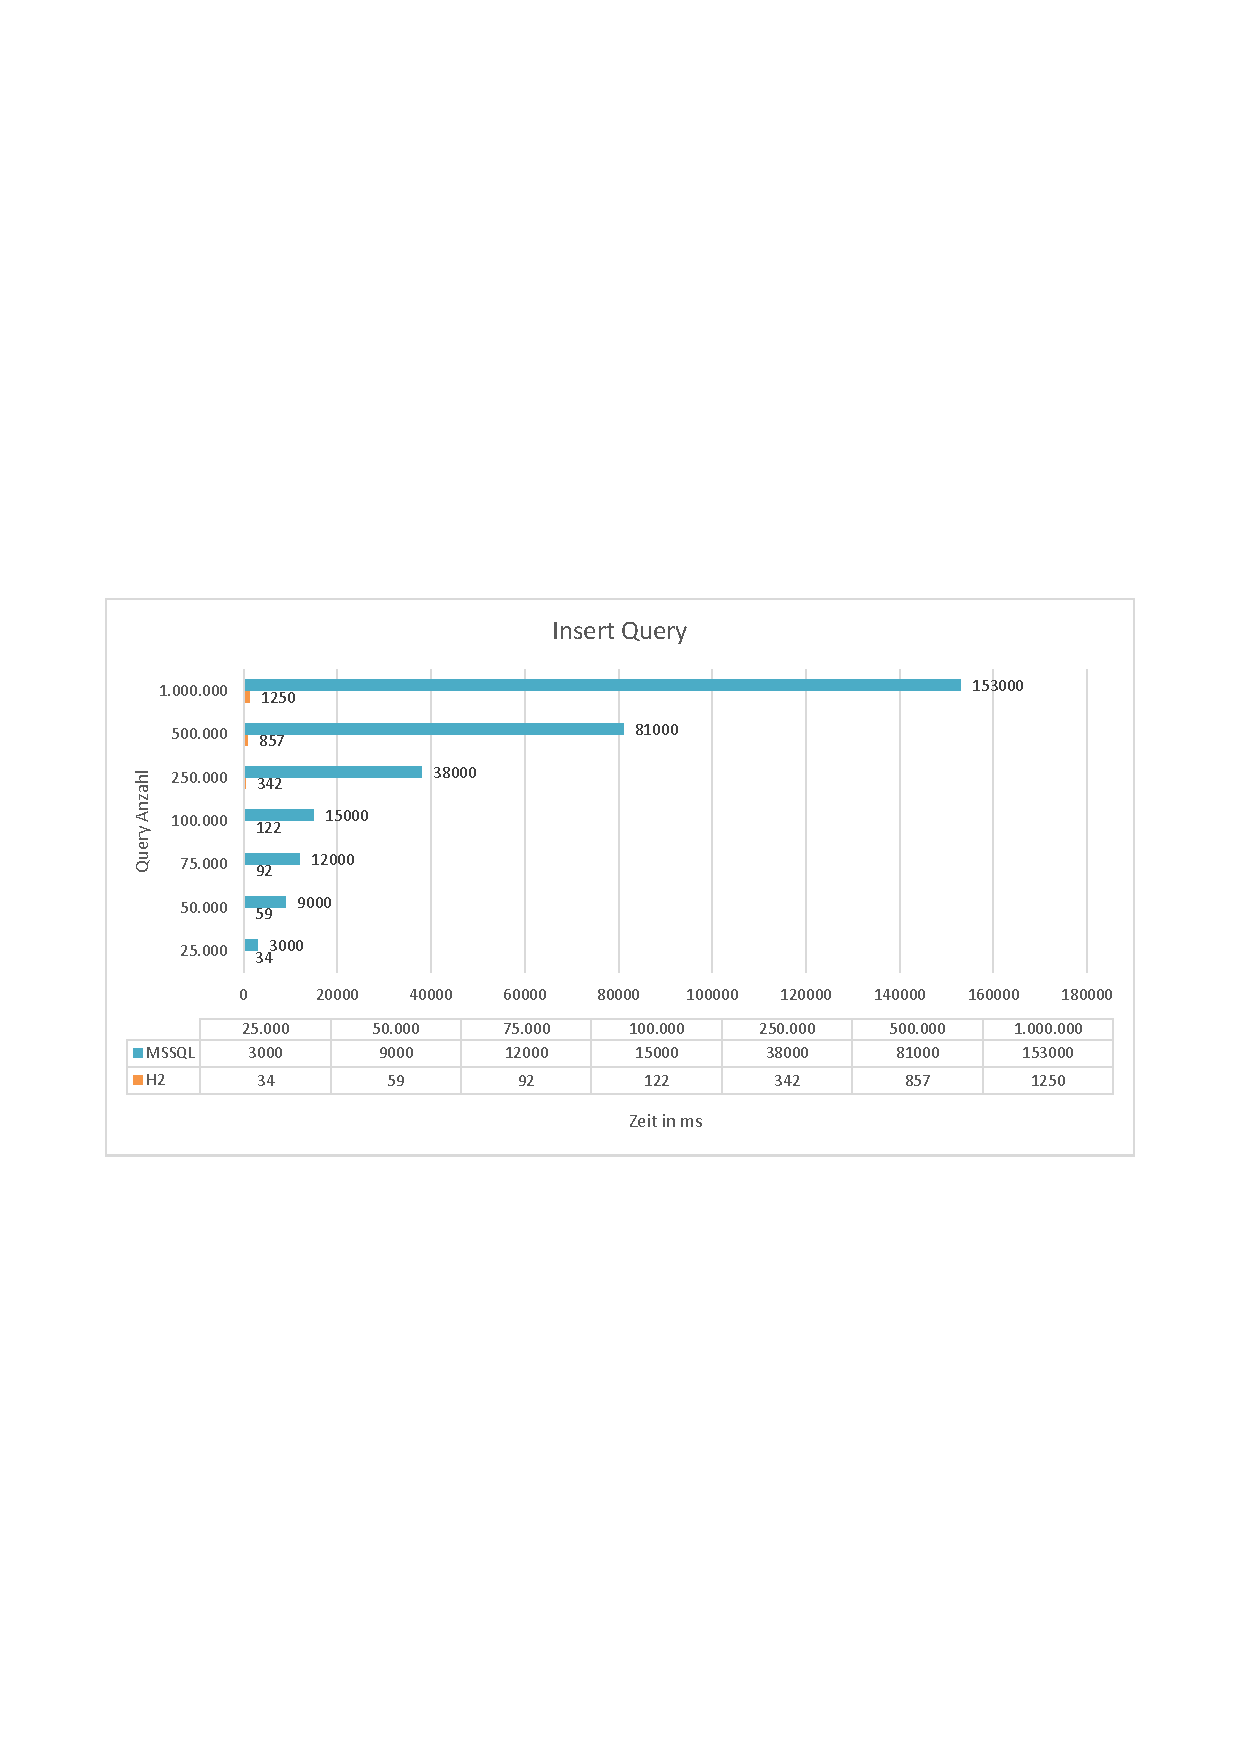
\includegraphics[width=0.5\textwidth]{charts/insert.pdf}}
\caption{Abfragegeschwindigkeit Vergleich}
\label{ergebniss_vergleich}
\end{figure}

Die Ergebnisse der Tests zeigen, dass die H2-Datenbank bei den durchgeführten Tests deutlich schneller als die MSSQL Datenbank ist. Der H2 ist bei SELECT-Anweisungen, um den Faktor 37 schneller. Bei Update-Anweisungen sogar um den Faktor 117. Ebenso bei Insert-Anweisungen, die einen Unterschied um den Faktor 124 aufweisen. Daraus lässt sich ableiten, dass die H2-Datenbank durch ihre In-Memory-Tabellen deutlich an Geschwindigkeit, im Gegensatz zu herkömmlichen Datenbanken, gewinnt. Diese Geschwindigkeit wird zum Teil durch den Verzicht auf Persistenz erlangt. Würde die Datenbank ihre Daten zur Sicherung auf die Festplatte schreiben, müsste bei Schreiboperationen mit Performance-Verschlechterungen gerechnet werden. Im vorliegenden System, welches fast nur Leseoperationen durchführt, stellt die mangelnde Persistenz allerdings kein großes Defizit dar. Ausschlaggebend für die Schnelligkeit ist allerdings die Nutzung des Hauptspeichers als Speichermedium. Dessen Gebrauch könnte allerdings in der Zukunft aufgrund der immer größer werdenden Datenmengen ein Problem darstellen.  

%% ===========================
\section{Ausblick}
\label{ch:Ergebnis:sec:Ausblick}
%% ===========================

Mit der Umsetzung des in der Arbeit beschriebenen Systems steht eine performante Lösung bereit, die eine Bewertung der Ausprägung von Beziehungen zwischen Personen aus einem CRM-System ermöglicht.

Die Bewertung der Beziehungen beruht derzeit lediglich auf der Anzahl von Verbindungsmerkmalen. Dementsprechend wird nur die Häufigkeit gewertet. Um die Bewertung einer Beziehungsausprägung genauer feststellen zu können, werden zusätzliche Regeln benötigt. Diese Regeln sollten auf psychologischen Erkenntnissen und Erfahrungswerten aufbauen. Durch Regeln ließe sich die Aussagekraft von Ergebnissen weiter steigern. Beispielsweise sind kommunikative Kontakte wie Telefonate oder E-Mail Verkehr, kein Indikator für Vertrauen. Die Einsicht in vertrauliche Dokumente setzt dagegen eine engere Zusammenarbeit bzw. Vertrauen voraus. Dies sollte somit stärker gewichtet werden. 

Neben festen Regeln in der Anwendungslogik könnten Gewichtungsprofile für die Nutzer umgesetzt werden. Ein Profil stellt in diesem Fall eine Voreinstellung der Gewichtungen dar. Demnach würde jedes Profil eine andere Charakteristik in der Abfrage darstellen. Zu diesen Profilen sollte eine Beschreibung beiliegen, die dem Nutzer den Zweck der Gewichtung näher bringt. Dadurch könnten sinnvolle Anpassungen auch durch Mitarbeiter ohne entsprechendes Fachwissen über Beziehungen vorgenommen werden.

Weiterhin könnten durch Vertriebsmitarbeiter mithilfe des Systems individuell unterstützt werden. Dazu werden zusätzliche Informationen über den Wert eines Kunden benötigt. Unter den Kunden müsste wie bei den Beziehungen ein Ranking aufgestellt werden. Nun könnten die Rankings auf Diskrepanzen verglichen werden. Auf diese Weise könnten zu große Unterschiede im betriebenen Aufwand und gewonnen Nutzen entdeckt werden. Weiterhin könnten Rankings in umgekehrter Folge durchgeführt werden. Dadurch könnten Kundenbeziehungen auf mangelhafte Kundenpflege hin untersucht werden. Dazu müsste lediglich eine Anpassung an der SQL-Abfrage vorgenommen werden.

Überdies könnten Ergebnisse verschiedener Personen verglichen werden. Der Vergleich könnte dabei unter Personen aus einer Gruppe oder aus selbst erstellten Personenkonstellationen erfolgen. Auf Vertriebsmitarbeiter angewandt könnte überprüft werden, ob die Verteilung der Kunden auf einzelne Mitarbeiter effizient gestaltet ist. Beispielsweise läse sich damit feststellen, ob zu viele Mitarbeiter sich unwissentlich auf denselben Kunden konzentrieren.

Eine andere weiterführende Möglichkeit wäre die Hinzunahme von Darstellungen, die eine Entwicklung der Beziehungen über die Zeit hinweg zeigen. Liniendiagramme wären dabei eine geeignete Form der Visualisierung, da sich mit ihnen zeitliche Abläufe gut darstellen lassen. Der Datenbestand bietet die Möglichkeiten dies umzusetzen, allerdings müssen entsprechende Abfragen und Darstellungen implementiert werden.  
